\documentclass[12pt,oneside]{article}
\usepackage{!sty/SBNart}
\usepackage{!sty/SBNsh}

%-------------------------------------------------------------------------------
% Info:
%-------------------------------------------------------------------------------
% *** Header:
\newcommand{\HdrL}{\normalfont \textsc{On Stability} }%{ \normalfont \textsc{ELEC5508-2016S} }   
\newcommand{\HdrC}{}%{ \normalfont Course Outline}
%
% *** Title (\htitle)
\newcommand{\TopL}{}
\newcommand{\TopR}{}
\newcommand{\midl}{Stability of the Linear Circuits}
\newcommand{\BotR}{By Behzad Nouri\\[4pt]Last-Update: \today}
%
%-------------------------------------------------------------------------------
\begin{document}
\isCUtitlefalse
\htitle{}{}
%%-------------------------------------------------------------------------------
% Title W. Photo  -- Table of contents + colored
%-------------------------------------------------------------------------------


%-------------------------------------------------------------------------------
% Title + Photo:
%-------------------------------------------------------------------------------
\vspace{2cm}
{\color[rgb]{0,0,0.4}%{0,0.071,0.5}
\begin{singlespace}
\begin{center}
\mbox{\colorbox[rgb]{0.85,0.85,0.85}{%{0.85,0.85,0.85}{
\begin{minipage}[h]{0.85\textwidth} 
\HRule 
%--------------------------------------------------------
{\flushleft {\Huge \textbf{Teaching Dossier}}}\\
%--------------------------------------------------------
\HRule\\[3pt]
\begin{minipage}{0.4\textwidth}
\begin{flushleft} 
%--------------------------------------------------------
{\Large \textsc{\textbf{S.-Behzad Nouri}} }\\ \vspace{14pt}
{\large {Electronics Department} }\\ \vspace{6pt}
{\large {Carleton University} }\\\vspace{6pt}
{\textbf{email:}~~\href{mailto:bnouri@gmail.com}{\underline{bnouri@gmail.com}}}\\
%--------------------------------------------------------
\end{flushleft}
\end{minipage}
\begin{minipage}{0.4\textwidth}
\begin{flushright}
%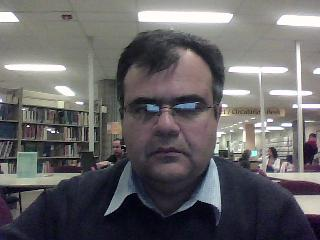
\includegraphics[trim=0.5in 0in 0in 0in, scale=0.5]{sbn09}
%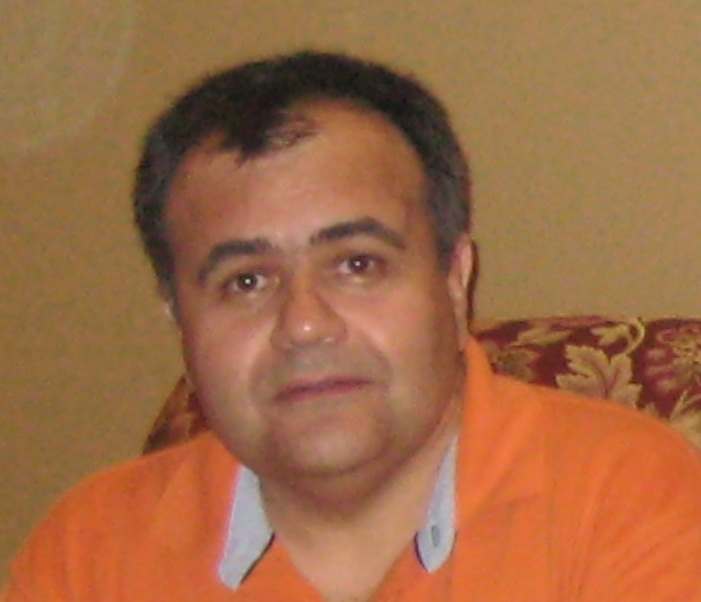
\includegraphics[trim=0.5in 0in 0in 0in, scale=0.2]{sbn11-1}
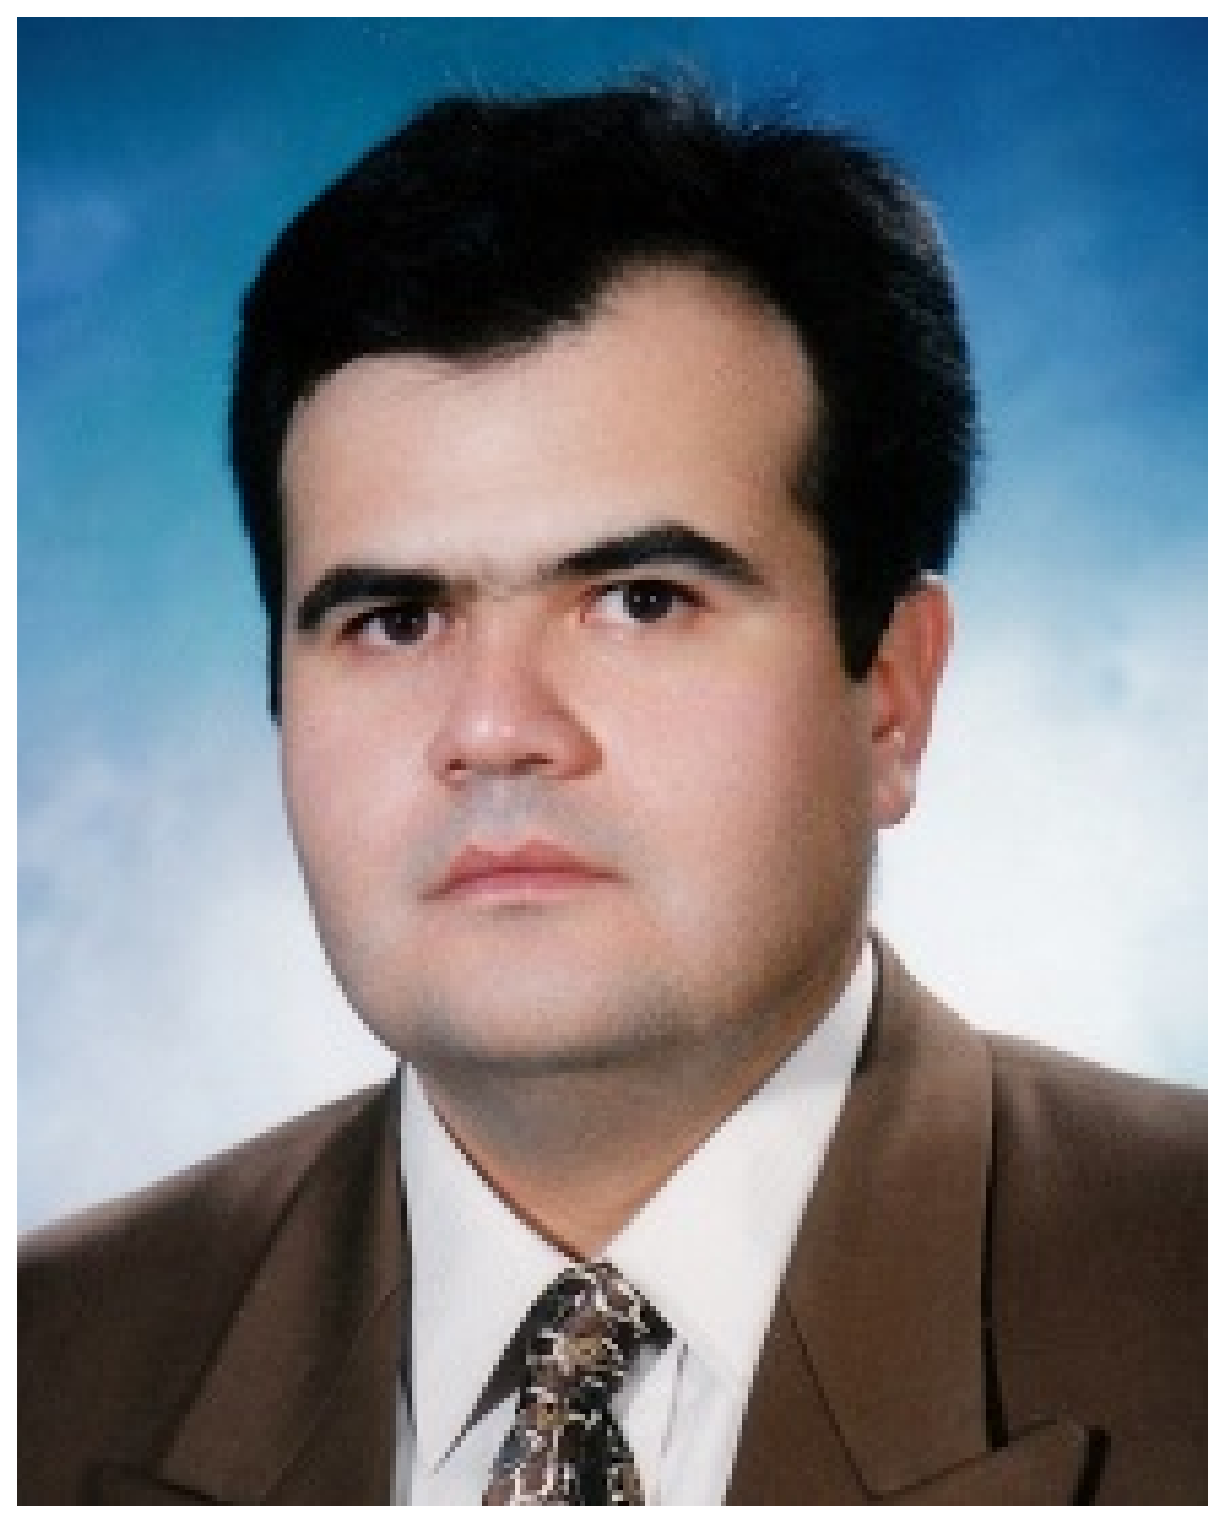
\includegraphics[trim=0.5in 0in 0in 0in, scale=0.12]{!opt/bn/sbn02c.eps}
\vspace{2pt}
\end{flushright}
\end{minipage}
\HRule 
\end{minipage} 
}} %\mbox
\end{center}
\end{singlespace}}



%-------------------------------------------------------------------------------
% Table of contents + colored
%-------------------------------------------------------------------------------
\begin{center}
%{\Large \textsc{\textbf{Cygwin~~Helps}} }\\ \vspace{14pt}  
\mbox{\colorbox[rgb]{0.92,0.92,0.92}{%{0.85,0.85,0.85}{
\begin{minipage}{0.75\textwidth}
\noindent \HRuleGray
\vspace{-12pt}
{\footnotesize \tableofcontents}
\noindent \HRuleGray
\end{minipage} }} %\mbox
\end{center}
\newpage

%---- End -------
\toc
%-------------------------------------------------------------------------------
% Title for Technical Note:
%-------------------------------------------------------------------------------
\rem{ % Simple Title for the Short Notes
	\mbox{}
	\begin{singlespace}
	\centering
	\textbf{\large Research Ideas}\\[6pt]
	\textbf{Behzad~Nouri}\\[4pt]
	Date:~August 23, 2016 %\today
	\end{singlespace}
} %rem
%-------------------------------------------------------------------------------

%-------------------------------------------------------------------------------
\section*{Entrance} \label{sec:entree}
%-------------------------------------------------------------------------------
This is a template!

%-------------------------------------------------------------------------------
\section{Introduction} \label{sec:intro}
%-------------------------------------------------------------------------------
Introduction goes here!
%
%-------------------------------------------------------------------------------
\section{Useful Command} \label{sec:useful}
%-------------------------------------------------------------------------------
This is as section with its own subsections including the fig.~\ref{fig:1}.
%-------------------------------------------------------------------------------
\subsection{Insert Figures} \label{sec:fig}
%-------------------------------------------------------------------------------
This is an example how a figure can be included in the \LaTeX file. The graphic formats including .png, *.jpg, *.pdf, and *.eps can be used.
\begin{figure}[!ht] 
\centering
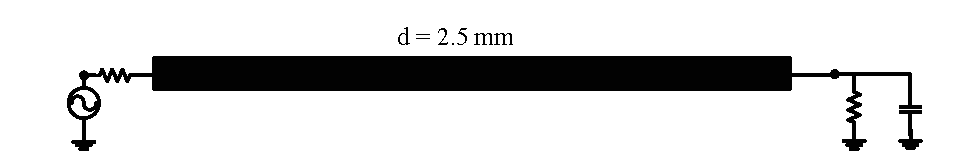
\includegraphics[trim=0in 0in 0in 0in, , clip=true, keepaspectratio=true, width=31pc]{Figs0/LinTL1.eps}
\caption{Linear transmission line circuit model.} 
\label{fig:1}
\end{figure} 
%
%
%
%-------------------------------------------------------------------------------
\newpage
%% Biblio:
\addcontentsline{toc}{section}{Bibliography}
\bibliography{K:/XXKK/zSBN-I/zIEEE_Biblio/nouri}
%-------------------------------------------------------------------------------


%-------------------------------------------------------------------------------
% % Appendices:
\newpage    
\appendix
%-------------------------------------------------------------------------------
\section{Some Fancy Stuff} \label{app:fancy}
%-------------------------------------------------------------------------------
The \verb@siunitx.sty@ package greatly simplifies TeXing when writing scientific documents, where units and numbers are a big part of the writing. This package adds commands like:\\
\SI{10}{\henry} \\
\num{+-2,345},  \num{1ie10},  \num{+-i2,345e13} \\
\SI{10}{\Omega}, \SI{30}{\ohm}, 40~\si{\ohm}\\
\si{\kilogram\metre\per\second} \\
\si{\radian/\second}\\

\par \noindent Or, as shown in the following below.
\begin{singlespace}
\begin{center}
\begin{tabular}{|c|c|c|}
\hline
Name              & Notation            & \verb@\si@  \\ 
                  &                     & command\\ \hline
ampere            & \si{\ampere}        & \verb@\si{\ampere}@ \\ \hline 
centimeter        & \si{\centi\metre}   & \verb@\si{\centi\metre}@\\ \hline
Angstrom          & \si{\angstrom}      & \verb@\si{\angstrom}@\\ \hline  
degree Centigrade & \si{\degreeCelsius} & \verb@\si{\degreeCelsius}@\\ \hline
kelvin            & \si{\kelvin}        & \verb@\si{\kelvin}@\\\hline 
Henry             & \si{\henry}         & \verb@\si{\henry}@\\\hline  
Second            & \si{\second}        & \verb@\si{\second}@\\ \hline     
Volt:             & \si{\volt}          & \verb@\si{\volt}@\\ \hline        						
electron volt     & \si{\electronvolt}  & \verb@\si{\electronvolt}@\\ \hline
Farad             & \si{\farad}         & \verb@\si{\farad}@\\ \hline
meter             & \si{\meter}         & \verb@\si{\meter}@ \\ \hline
Ohm               & \si{\ohm}           & \verb@\si{\ohm}@ \\ \hline
\end{tabular}
\end{center}
\end{singlespace}
%-------------------------------------------------------------------------------
\end{document}
%-------------------------------------------------------------------------------

